\chapter{$\Lambda$ Production In and Out-of Jets: Analysis Overview}

This chapter will provide a high-level description of the main analysis topic of this dissertation: using the \lmb baryon to investigate the origins of strangeness enhancement in \pPb collisions. First, the goal of this analysis will be clearly stated, along with the steps needed to acheive this goal. Then, each step will be described with more detail, including justification. Finally, the analysis will be summarized, and the next chapter will describe the analysis in more detail.

\section{Objective}
While the phrase ``origins of strangeness enhancement'' is concise, it lacks the specificity required to bring the analysis to fruition. In order to make 


\subsection{Motivation}
\label{motivation}
Recent studies have shown that the ratio of the yield of \lmb baryons to charged pions differs between pp, \pPb and \PbPb collisions, specifically in the mid-\pt region of 1-4 \GeVc.  Additionally, similar studies have seen an increase in the $\Lambda/(\pi^{+} + \pi^{-})$ yields as a function of charged particle multiplicity in \pPb collisions. The origin of this increase is still unknown.

By performing angular correlations of a high $p_T$ trigger hadron with an associated $\Lambda$ (or charged hadron as a proxy for a pion) in p-Pb events, we are able to separate out $\Lambda$ baryon production into three distinct kinematic regions:
\begin{itemize}
\item The near-side peak of the correlation, corresponding to jet-like production with no medium interactions,
\item The away-side peak of the correlation, corresponding to jet-like production with possible medium interaction, and
\item The uncorrelated pairs, corresponding to the ``underlying event'' or soft production within the medium.
\end{itemize}

A h-h $\Delta\varphi$ distribution with these regions highlighted is shown in Figure \ref{fig:dphi_regions}. Using this technique, we can then determine the (h-)$\Lambda$/(h-)h ratio in each of this regions as a function of multiplicity to gain insight to the origins of the enhancement.

\begin{figure}
\centering
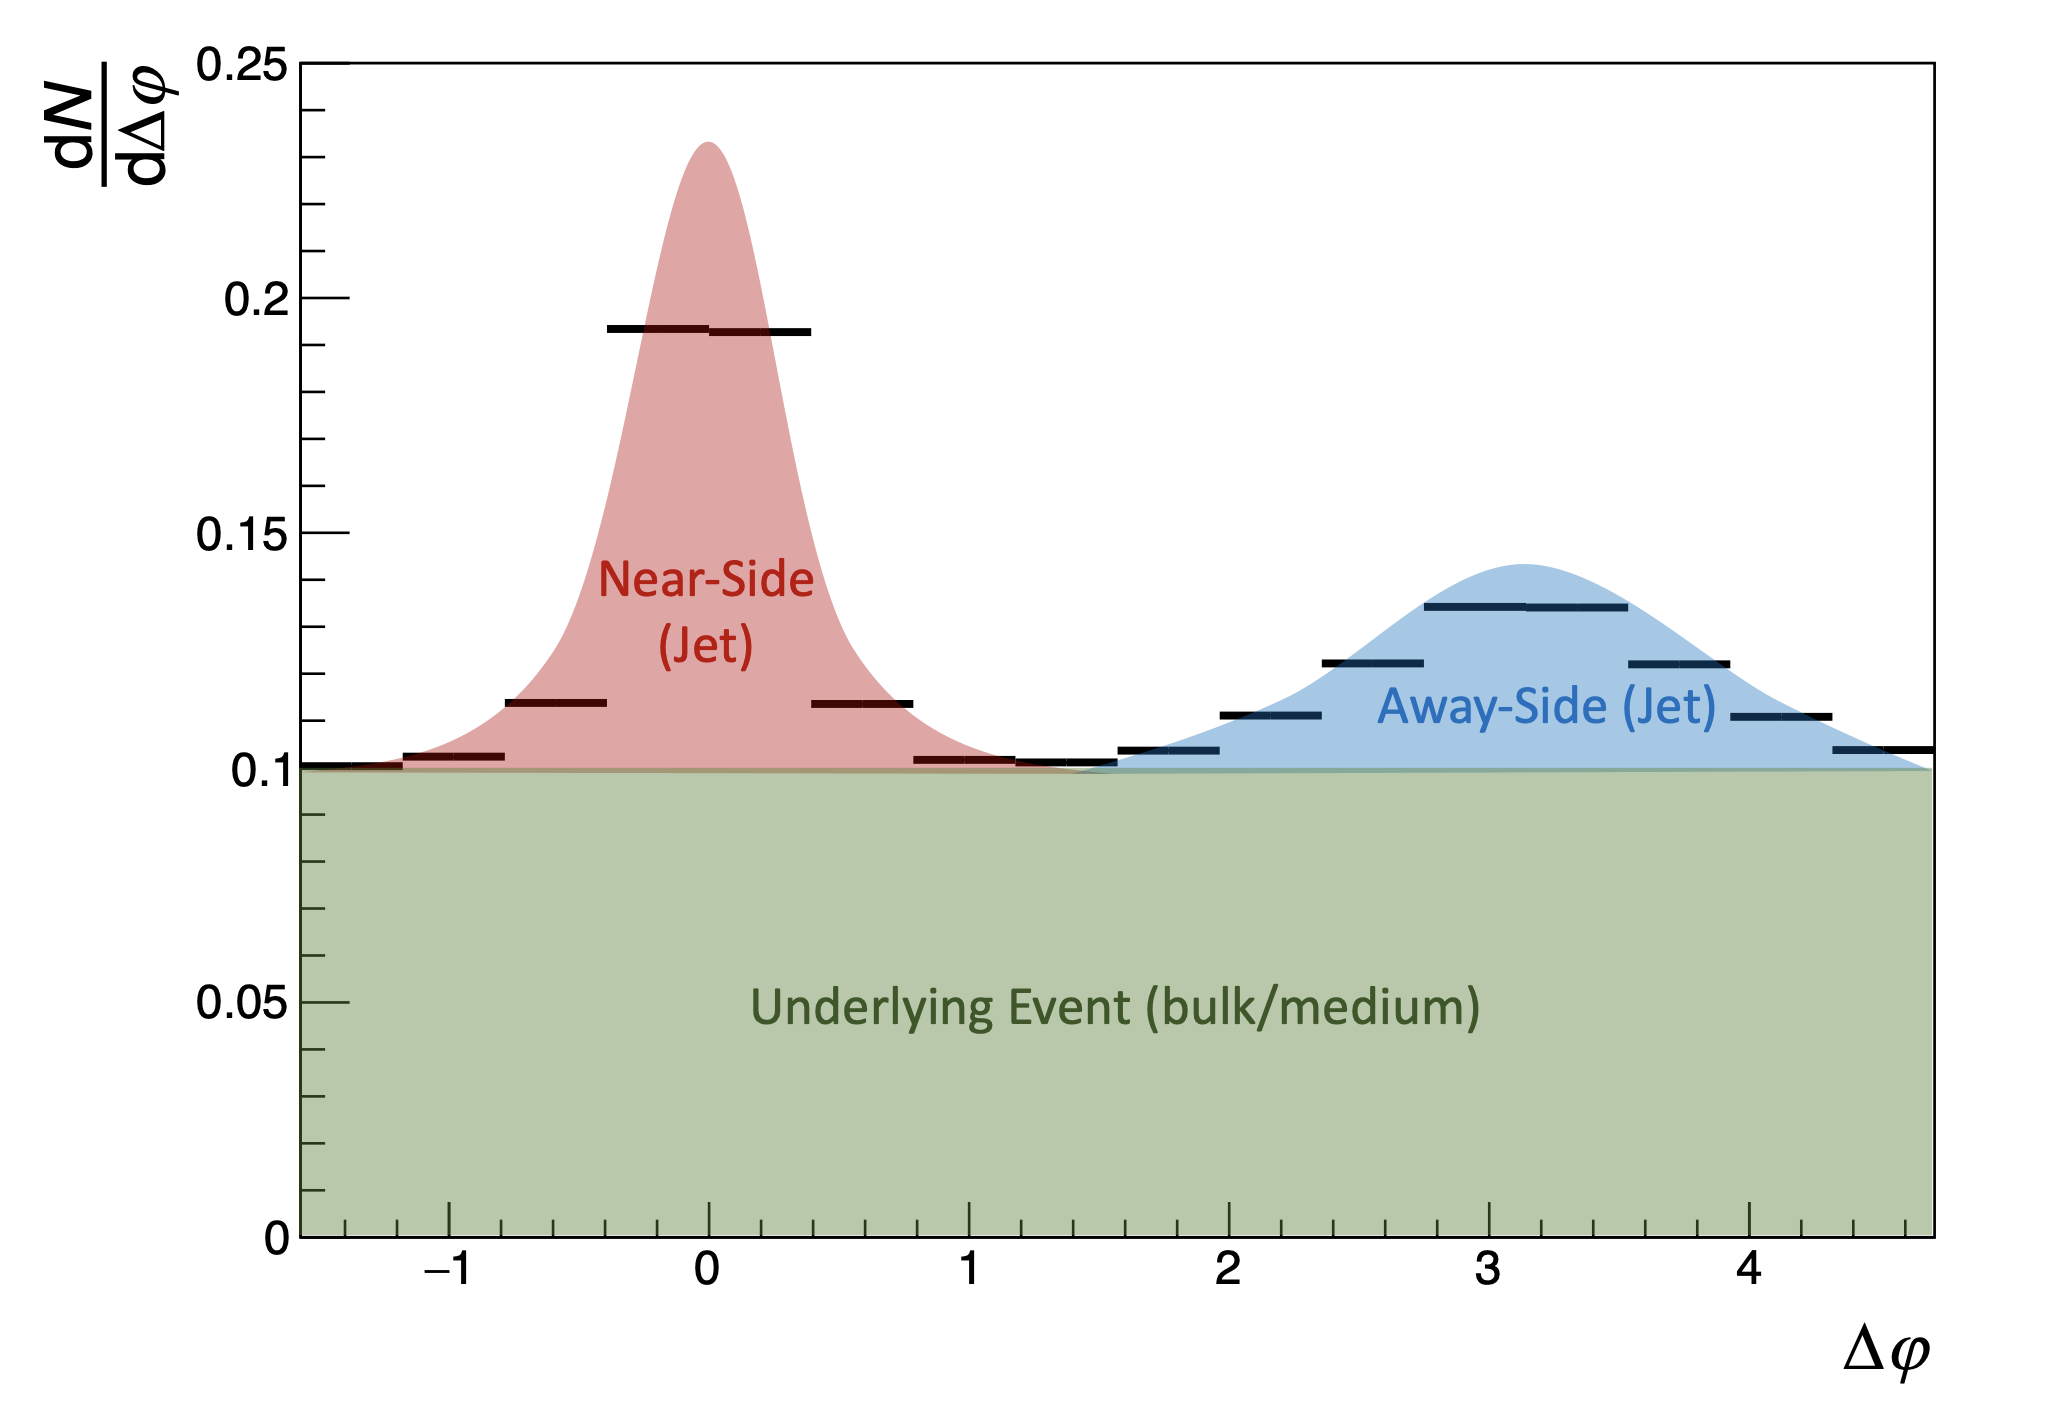
\includegraphics[width=4in]{figures/analysis/dphi_regions.png}
\caption{A h-h $\Delta\varphi$ distribution taken from this analysis with the near-side, away-side, and uncorrelated regions highlighted.}
\label{fig:dphi_regions}
\end{figure}

For this study, 1-d $\Delta\varphi$ angular correlations of jet-like $h-\Lambda$ and $h-h$ pairs were measured in p-Pb events independently for three multiplicity bins (0-20\%, 20-50\%, 50-80\%), and the final ratios of yields of correlated pairs were compared to study the onset of this enhancement. 





